\speciestitle{Chlorine Monoxide}{ClO}{ClO}{%
\item[Useful range:] 147--1.0\,hPa
\item[Contact:] Michelle Santee, \email{Michelle.L.Santee@jpl.nasa.gov}}

\subsection{Introduction}

As in previous versions, in \thisv the standard ClO product is derived
from radiances measured by the radiometer centered near 640\,GHz.  ClO
is also retrieved using radiances from the \mbox{190-GHz} radiometer,
but those data have poorer precision and larger biases and are not
used in the standard ClO product.  The quality and reliability of the
version~2 (v2.2) Aura MLS ClO measurements were assessed in detail by
\citet{SanteeEtal:2008:ClO}.  The ClO product was significantly
improved in v3.3\emph{x}/v3.4\emph{x} \citep{EOSMLSV33V34Quality}; in
particular, the substantial (\mytexttilde0.1--0.4\,ppbv) negative
bias present in the v2.2 ClO values at retrieval levels below (i.e.,
pressures larger than) 22\,hPa was mitigated to a large extent,
primarily through retrieval of CH\cs3Cl, which was a new MLS product
in v3.3\emph{x}/v3.4\emph{x}.  The ClO retrieval was largely unchanged
over much of the profile in \prevv, and the \thisv retrieval does not
depart dramatically from \prevv, although the biases present at the
lowest retrieval levels have been further reduced (see
Section~\ref{sec:cloBias}).  The MLS \thisv ClO data are
scientifically useful over the range 147 to 1\,hPa.  A summary of the
estimated precision, resolution (vertical and horizontal), and
systematic uncertainty of the \thisv ClO measurements as a function of
altitude is given in Table~\ref{tab:ClOSummary}.

\subsection{Resolution}
\onestandardavk{ClO}{ClO}%

The resolution of the retrieved data can be described using
``averaging kernels'' \citep[e.g.,][]{Rodgers:2000}; the
two-dimensional nature of the MLS data processing system means that
the kernels describe both vertical and horizontal resolution.
Smoothing, imposed on the retrieval system in both the vertical and
horizontal directions to enhance retrieval stability and precision,
degrades the inherent resolution of the measurements.  Thus, although
ClO measurements are reported at six pressure levels per decade change
in pressure (spacing of \mytexttilde2.7\,km), the vertical resolution
of the \thisv ClO data as determined from the full width at half
maximum of the rows of the averaging kernel matrix shown in
Figure~\ref{fig:AvkClO} is \mytexttilde3--4.5\,km throughout the
retrieval range (with a mean of \mytexttilde3.5\,km).  As in \prevv,
in \thisv the averaging kernels are sharply peaked at all levels,
including 147\,hPa.  Thus, although some degree of overlap is present,
the 147\,hPa surface provides independent information in \thisv.
Figure~\ref{fig:AvkClO} also shows horizontal averaging kernels, from
which the along-track horizontal resolution is determined to be
\mytexttilde300--500\,km over most of the vertical range.  The
cross-track resolution, set by the width of the field of view of the
\mbox{640-GHz} radiometer, is \mytexttilde3\,km.  The along-track
separation between adjacent retrieved profiles is 1.5{\degsym} great
circle angle (\mytexttilde165\,km), whereas the longitudinal
separation of MLS measurements, set by the Aura orbit, is
10{\degsym}--20{\degsym} over low and middle latitudes, with much
finer sampling in the polar regions.

\subsection{Precision}

\begin{figure}
\centering\includegraphics[width=8.4cm]{figures/ComparePrecision2Panel-ClO}
\caption{Precision of the (left) \thisv and (right) \prevv MLS ClO
  measurements for four representative days in different seasons (see
  legend).  Solid lines depict the observed scatter in nighttime
  (descending) measurements obtained in a narrow equatorial band (see
  text); dotted lines depict the theoretical precision estimated by
  the retrieval algorithm. The light grey vertical line marks
  0.1\,ppbv, the estimated single-profile precision over most of the
  recommended vertical range in both versions.}
\label{fig:ClOPrecProf}
\end{figure}

The precision of the MLS ClO measurements is estimated empirically by
computing the standard deviation of the descending (i.e., nighttime)
profiles in the 20{\degsym}-wide latitude band centered around the
equator.  For this region and time of day, natural atmospheric
variability should be negligible relative to the measurement noise.
As shown in Figure~\ref{fig:ClOPrecProf}, the observed scatter in the
data is virtually unchanged in \thisv, ranging from
\mytexttilde0.1\,ppbv over the interval 100--3\,hPa to
\mytexttilde0.2\,ppbv at 147\,hPa and \mytexttilde0.3\,ppbv at
1\,hPa.  The smoothing of the retrieval is turned off above 1\,hPa,
and as a consequence the precision worsens steeply above this level.
The scatter in the data is essentially invariant with time, as seen by
comparing the results for the different days shown in
Figure~\ref{fig:ClOPrecProf}.

The single-profile precision estimates cited here are, to first order,
independent of latitude and season, but of course the scientific
utility of individual MLS profiles (i.e., signal to noise) varies with
ClO abundance.  Outside of the lower stratospheric winter polar
vortices, within which ClO is often strongly enhanced, the
single-profile precision exceeds typical ClO mixing ratios,
necessitating the use of averages for scientific studies.  Precision
can generally be improved by averaging, with the precision of an
average of $N$ profiles being 1/$\sqrt{N}$ times the precision of an
individual profile (although the actual standard error of the mean can
in some cases be even smaller \citep{TooheyAndVonClarmann:2013}).

The observational determination of the precision is compared in
Figure~\ref{fig:ClOPrecProf} to the theoretical precision values
reported by the Level~2 data processing algorithms.  The predicted
precision exceeds the observed scatter, particularly above 15\,hPa,
indicating that the vertical smoothing (regularization) applied to
stabilize the retrieval and improve the precision has a non-negligible
influence on the results at these levels.  Because the theoretical
precisions take into account occasional variations in instrument
performance, the best estimate of the precision of an individual data
point is the value quoted for that point in the L2GP files, but it
should be borne in mind that this approach slightly overestimates the
actual measurement noise.

\subsection{Accuracy}
\label{sec:cloacc}

The effects of various sources of systematic uncertainty (e.g.,
instrumental issues, spectroscopic uncertainty, and approximations in
the retrieval formulation and implementation) on the MLS \thisv ClO
measurements have been quantified through a comprehensive set of
retrievals of synthetic radiances; see \citet{SanteeEtal:2008:ClO} for
details of a similar analysis conducted on MLS v2.2 ClO data.  The
overall systematic uncertainty, or accuracy, is calculated by
combining (RSS) the contributions from both the expected biases and
the additional scatter each source of uncertainty may introduce into
the data.  In aggregate, the factors considered in these simulations
are estimated to give rise to a total systematic uncertainty ranging
from approximately 0.02 to 0.6\,ppbv, depending on the level, in the
MLS \thisv ClO data (see Table~\ref{tab:ClOSummary}).  These values
for the overall uncertainty in \thisv ClO, which are slightly larger
(poorer accuracy) at 100 and 147\,hPa than those estimated for the
\prevv data \citep[see][]{EOSMLSV4Quality}, do not take into account
the known biases in MLS ClO data at the lowest retrieval levels
discussed in the following subsection.

\subsection{Quantification and correction of biases in
  \prevv and \thisv}
\label{sec:cloBias}

As with other species retrieved from the MLS \mbox{640-GHz} receiver,
lower stratospheric signals for ClO are affected by water
vapor. Therefore, for the retrieval phase CorePlusR4AB14, which
includes ClO (see Table~\ref{tab:Phases}), water vapor is constrained
to the values from the MLS H\cs2O standard product.  As discussed in
Section~\ref{sec:H2OChanges}, the dry bias below the tropopause
present in earlier MLS data versions has been mitigated in \thisv.
Some of the differences between \thisv and \prevv ClO can thus be
attributed to the improvement in H\cs2O between the two versions.
Zonal-mean differences from \prevv are generally small (less than
10\%) except at the bottom of the retrieval range (68--147\,hPa),
where low ClO abundances lead to larger percent differences
(Figure~\ref{fig:zmcontourClO}).  Figure~\ref{fig:clov3v2bylat}
depicts \thisv and \prevv nighttime mixing ratios for a representative
day during winter (when ClO is enhanced in the sunlit polar lower
stratosphere) in both the Northern and Southern Hemispheres, and mean
daytime and nighttime vertical profiles from the two versions are
compared in the tropics and the Northern and Southern Hemisphere polar
regions for the same two days in Figure~\ref{fig:cloMeanProfs}; plots
for other days give similar results (not shown).  The two versions are
in very close agreement at higher levels, including around the
secondary peak in the ClO profile in the upper stratosphere
(Figure~\ref{fig:cloMeanProfs}).  In addition to the standard product
(derived from the \mbox{640-GHz} radiances),
Figure~\ref{fig:cloMeanProfs} includes results for the product
retrieved from the \mbox{190-GHz} radiances.  The very large negative
bias in \texttt{ClO-190} at its lowest retrieval levels (68--100\,hPa)
has been greatly reduced in \thisv; thus the two ClO products
correspond more closely now than they did in \prevv.  Nevertheless,
both continue to display non-negligible biases that need to be
corrected before being used in detailed quantitative studies (as was
the case for previous versions of the MLS ClO data).

\begin{figure}
  \begin{center}
      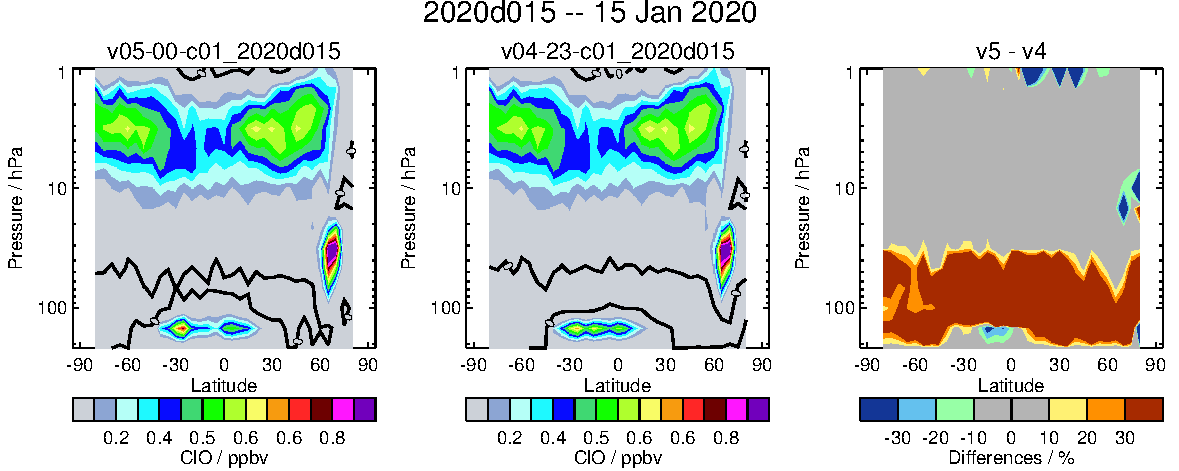
\includegraphics[width=10.0cm]{figures/Zm_ClO_2020d015}
      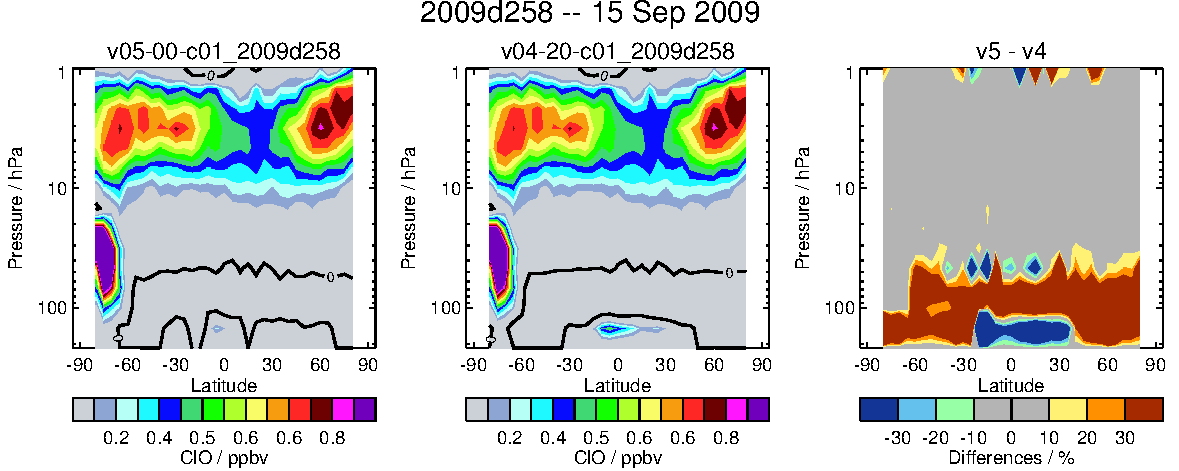
\includegraphics[width=10.0cm]{figures/Zm_ClO_2009d258}
  \end{center}
\caption{Zonal mean pressure-latitude cross sections of MLS daytime
  (ascending) ClO, for (left) \thisv, (middle) \prevv, and (right)
  their differences (\thisv minus \prevv, in percent).  No bias
  corrections have been applied.  Results from a representative day
  with strong ClO enhancement in the winter polar region are shown for
  (top panels) the Northern Hemisphere and (bottom panels) the
  Southern Hemisphere.  The black curves overlaid on the abundance
  panels (left and middle) mark the zero contour.}
\label{fig:zmcontourClO}
\end{figure}

\begin{figure}
  \begin{center}
 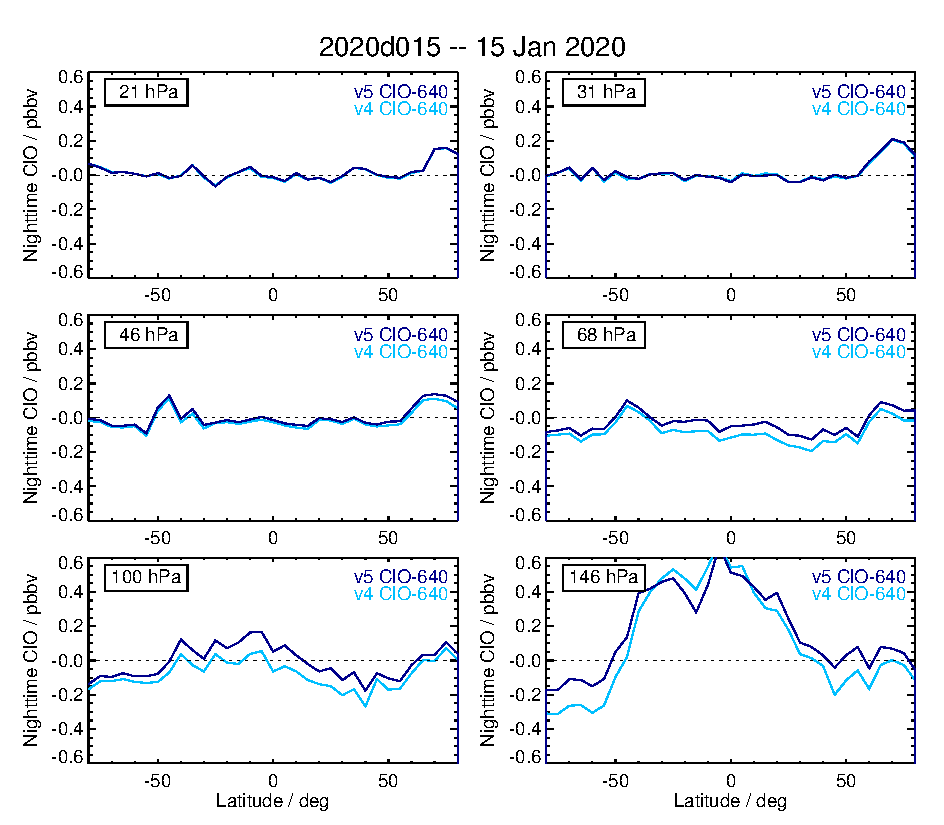
\includegraphics[width=0.48\linewidth]{figures/clov5v4bylat_ClO-640_2020d015}%
 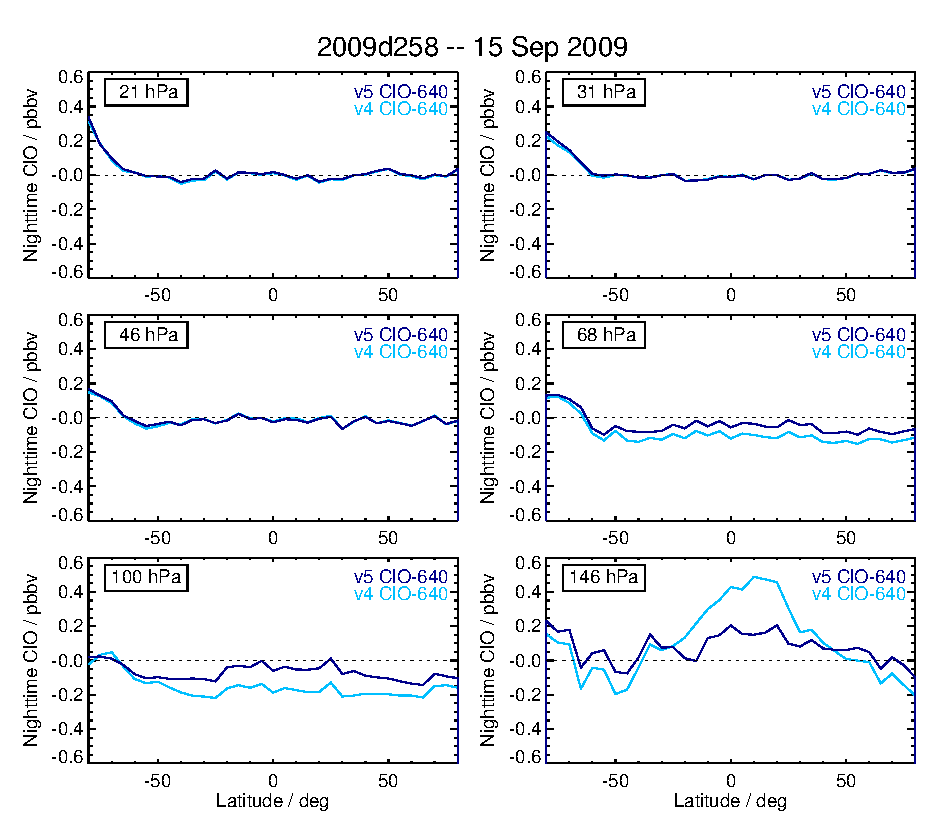
\includegraphics[width=0.48\linewidth]{figures/clov5v4bylat_ClO-640_2009d258}%
   \end{center}
\caption{Nighttime \thisv (dark blue) and \prevv (light blue) MLS ClO
  data as a function of latitude for the six lowest retrieval pressure
  surfaces (21--147\,hPa) for a representative day during winter in
  the Northern (left) and Southern (right) Hemispheres.}
\label{fig:clov3v2bylat}
\end{figure}

\begin{figure}
  \begin{center}   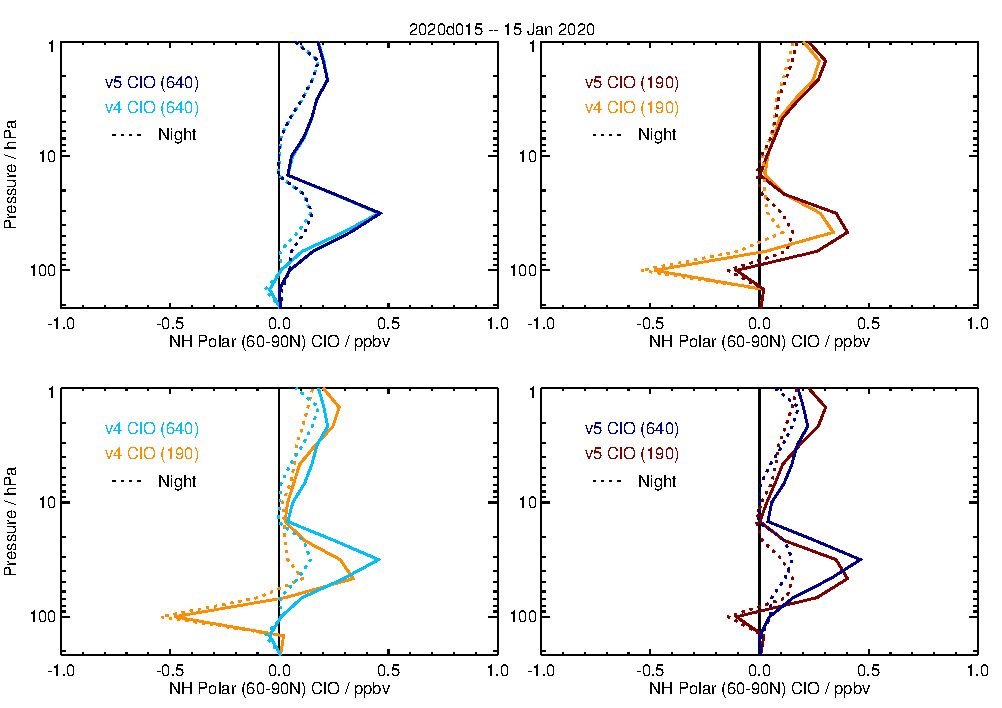
\includegraphics[width=0.48\linewidth]{figures/meanprofcomparison_ClO_2020d015_NHPolar}\hfill    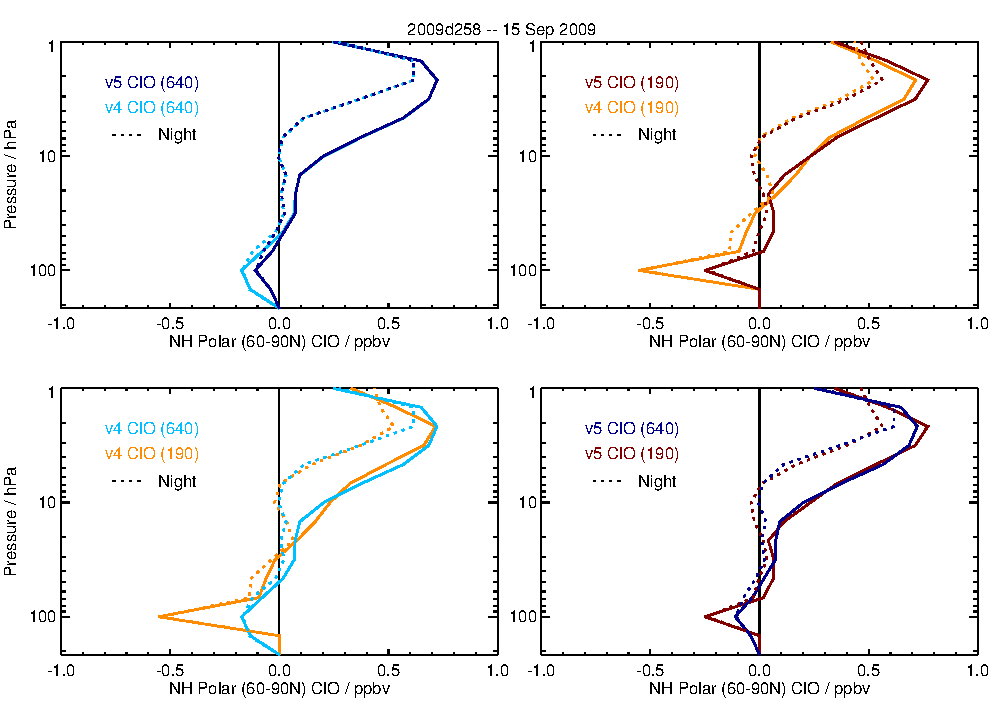
\includegraphics[width=0.48\linewidth]{figures/meanprofcomparison_ClO_2009d258_NHPolar}
  \end{center}
  \begin{center} 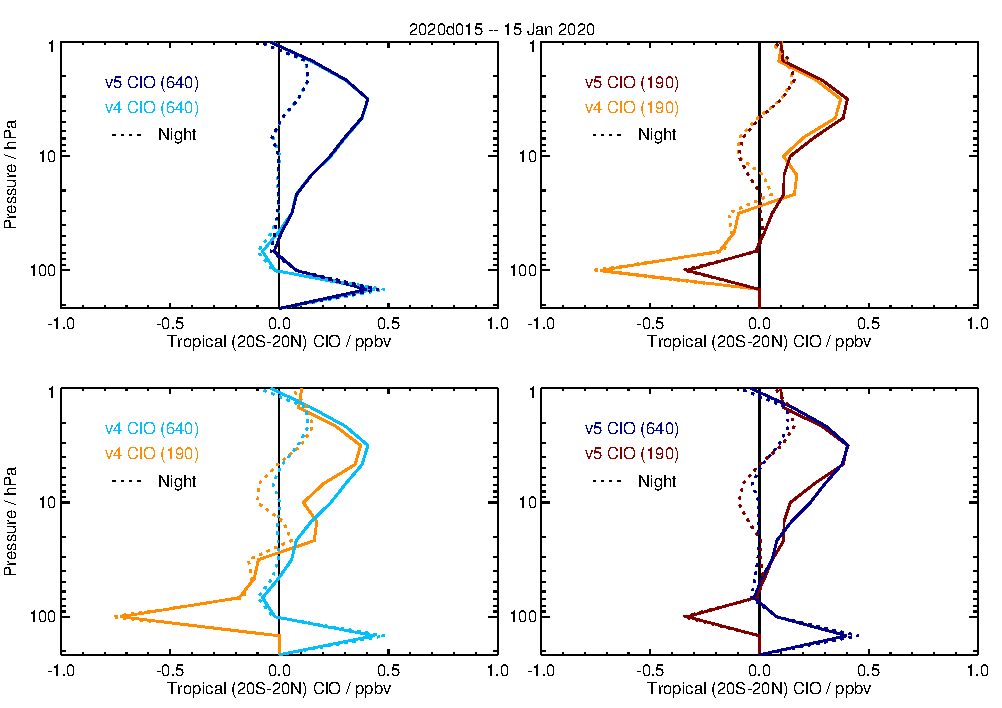
\includegraphics[width=0.48\linewidth]{figures/meanprofcomparison_ClO_2020d015_Tropical}\hfill 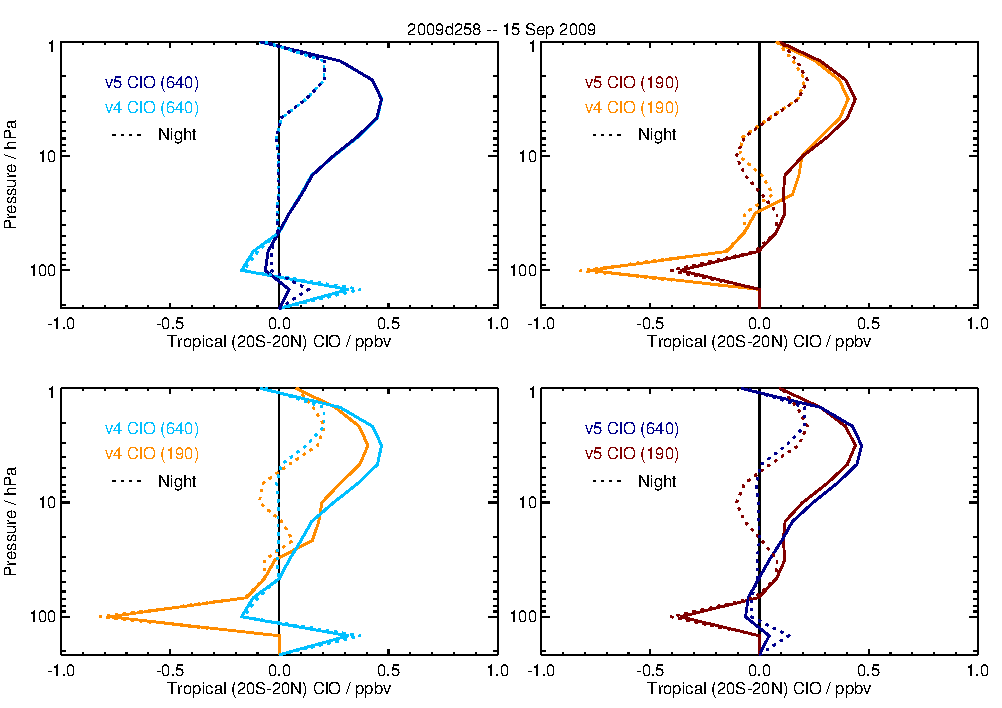
\includegraphics[width=0.48\linewidth]{figures/meanprofcomparison_ClO_2009d258_Tropical}
  \end{center}
  \begin{center}
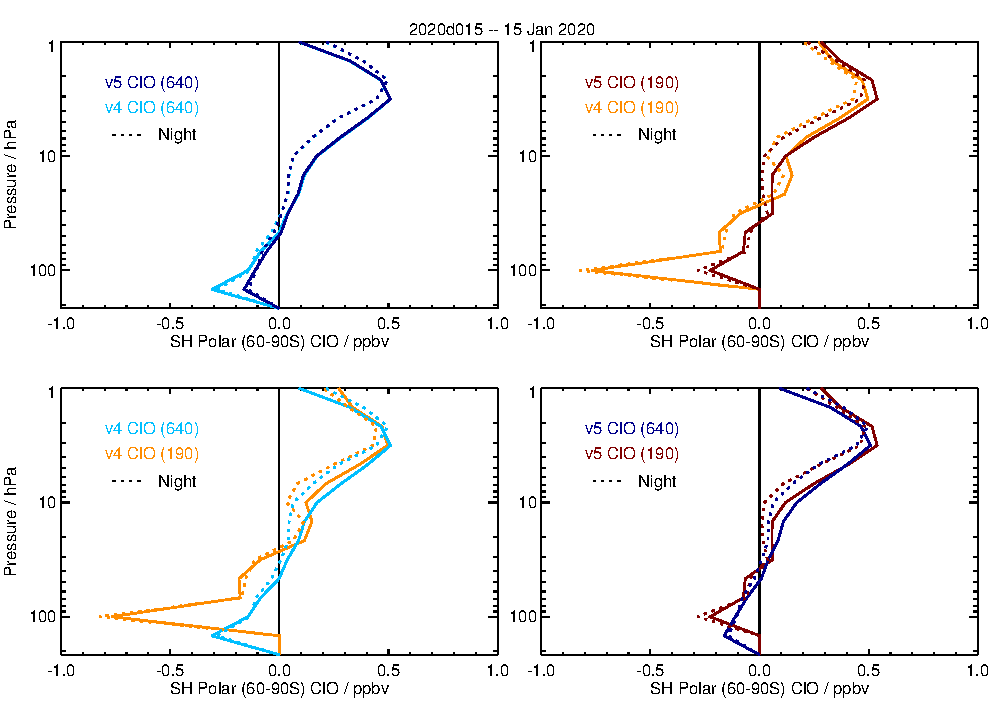
\includegraphics[width=0.48\linewidth]{figures/meanprofcomparison_ClO_2020d015_SHPolar}\hfill 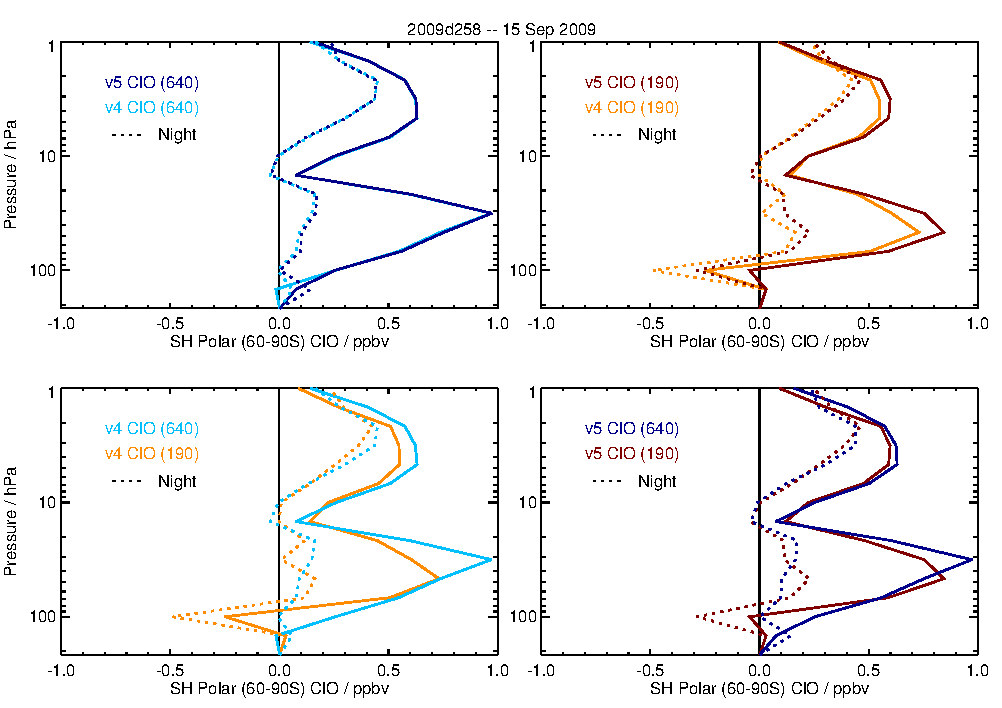
\includegraphics[width=0.48\linewidth]{figures/meanprofcomparison_ClO_2009d258_SHPolar}
  \end{center}
\caption{MLS \thisv (dark colors) and \prevv (light colors) profiles
  of \texttt{ClO-640} (blues) and \texttt{ClO-190} (reds) averaged
  over the Northern Hemisphere polar (top set), tropical (middle set),
  and Southern Hemisphere polar (bottom set) regions for a
  representative day during winter in the Northern (left side) and
  Southern (right side) Hemispheres.  Each set of plots contains four
  panels, comparing \thisv and \prevv \texttt{ClO-640} retrievals,
  \thisv and \prevv \texttt{ClO-190} retrievals, \prevv
  \texttt{ClO-640} and \texttt{ClO-190} retrievals, and \thisv
  \texttt{ClO-640} and \texttt{ClO-190} retrievals.  Solid lines show
  ascending (mainly daytime) and dashed lines show descending (mainly
  nighttime) averages.}
\label{fig:cloMeanProfs}
\end{figure}

Figures~\ref{fig:zmcontourClO}--\ref{fig:cloMeanProfs} show that the
differences between the two versions are larger at the lowest
retrieval pressure levels, where substantial biases present in \prevv
have been ameliorated in \thisv.  To investigate in more detail the
magnitude of and temporal variations in the bias in the \thisv MLS ClO
data and compare them to \prevv, we show in
Figure~\ref{fig:cloBiasByMonth} monthly zonal means of MLS nighttime
ClO measurements for pressure levels 147--46\,hPa.  Each panel
represents a calendar month; nighttime data taken during that month
over the period 2005--2020 have been binned and averaged in
5{\degsym}-wide latitude bands between
$\pm$85{\degsym}. Figure~\ref{fig:cloBiasByPress} is a similar plot
but encompasses all of the MLS nighttime ClO data (i.e., the
climatological annual mean over 2005--2020) for pressure levels
147--10\,hPa.  In both figures, bold colors represent \thisv data,
while corresponding pale colors represent \prevv data.  To guide the
eye, the global-mean annual-mean bias calculated over the
climatological period is indicated for each pressure level (horizontal
solid lines in the respective bold and pale colors).
Figures~\ref{fig:clov3v2bylat}, \ref{fig:cloBiasByMonth}, and
\ref{fig:cloBiasByPress} show that the magnitude, and at 100 and
147\,hPa even the sign, of the bias varies with latitude as well as
pressure.  At 46\,hPa, a negligible negative bias present in \prevv is
further reduced in \thisv.  At 68\,hPa, the small negative bias in
\prevv is considerably lessened but is still evident in \thisv.  At
100\,hPa, the substantial negative bias at higher latitudes (in both
hemispheres) is much smaller, but a slight positive bias is now seen
in the tropics.  At the latter two levels, the magnitude of the
global-mean bias decreased by about half between \prevv and \thisv.
At 147\,hPa, both the large negative bias in the polar regions and the
large positive bias at low latitudes are much smaller, such that the
strong latitude dependence at this level in \prevv has been somewhat
flattened in \thisv.  However, unlike at 68 and 100\,hPa, the global
mean bias has increased slightly at 147\,hPa in \thisv.  In contrast
to the strong altitude and latitude dependence of the ClO bias evident
in these plots, Figure~\ref{fig:cloBiasByMonth} reveals only slight
month-to-month variability in most places.

\begin{figure}
\centering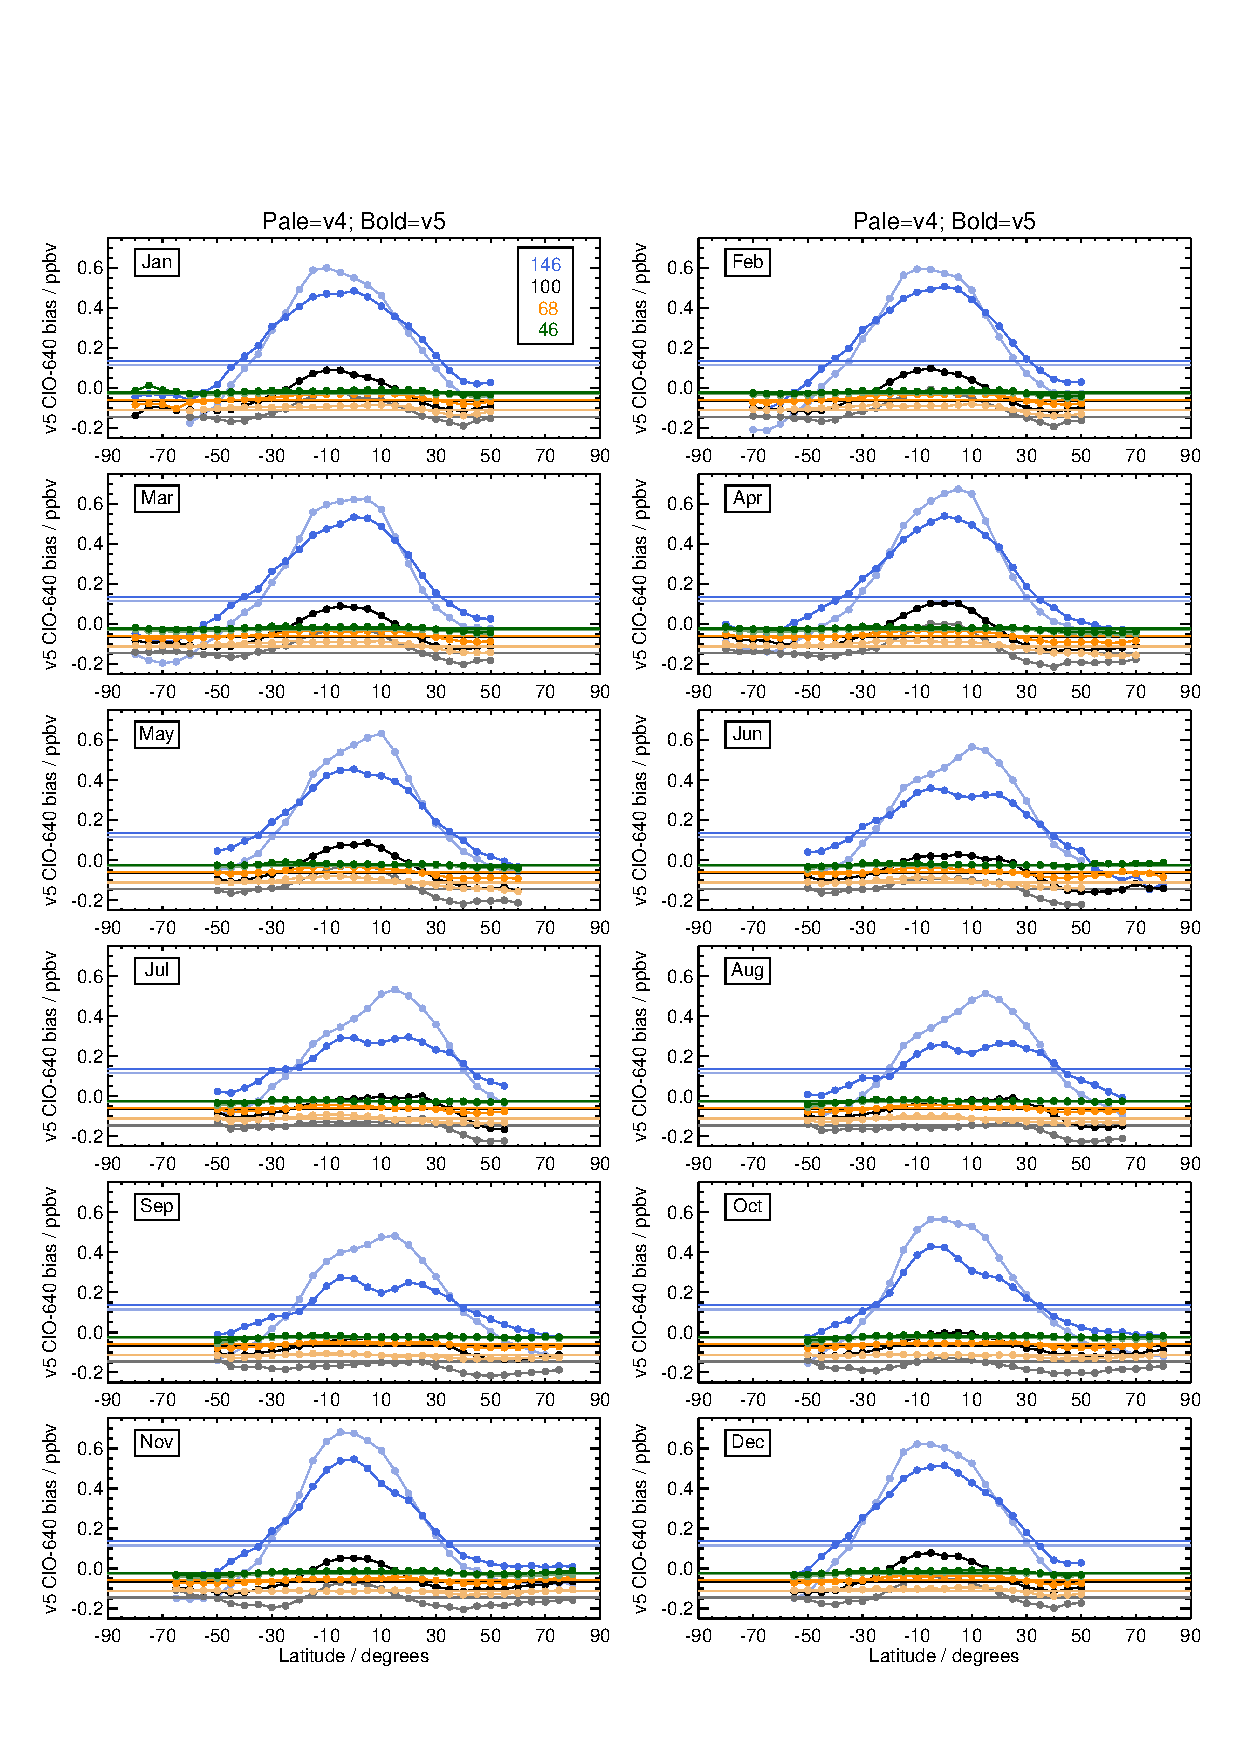
\includegraphics[width=\linewidth,clip=true,trim=0cm 1.5cm 0cm 3.0cm]{figures/plotBiasV5ByMonth-Clim_2020_ClO640}
%\centering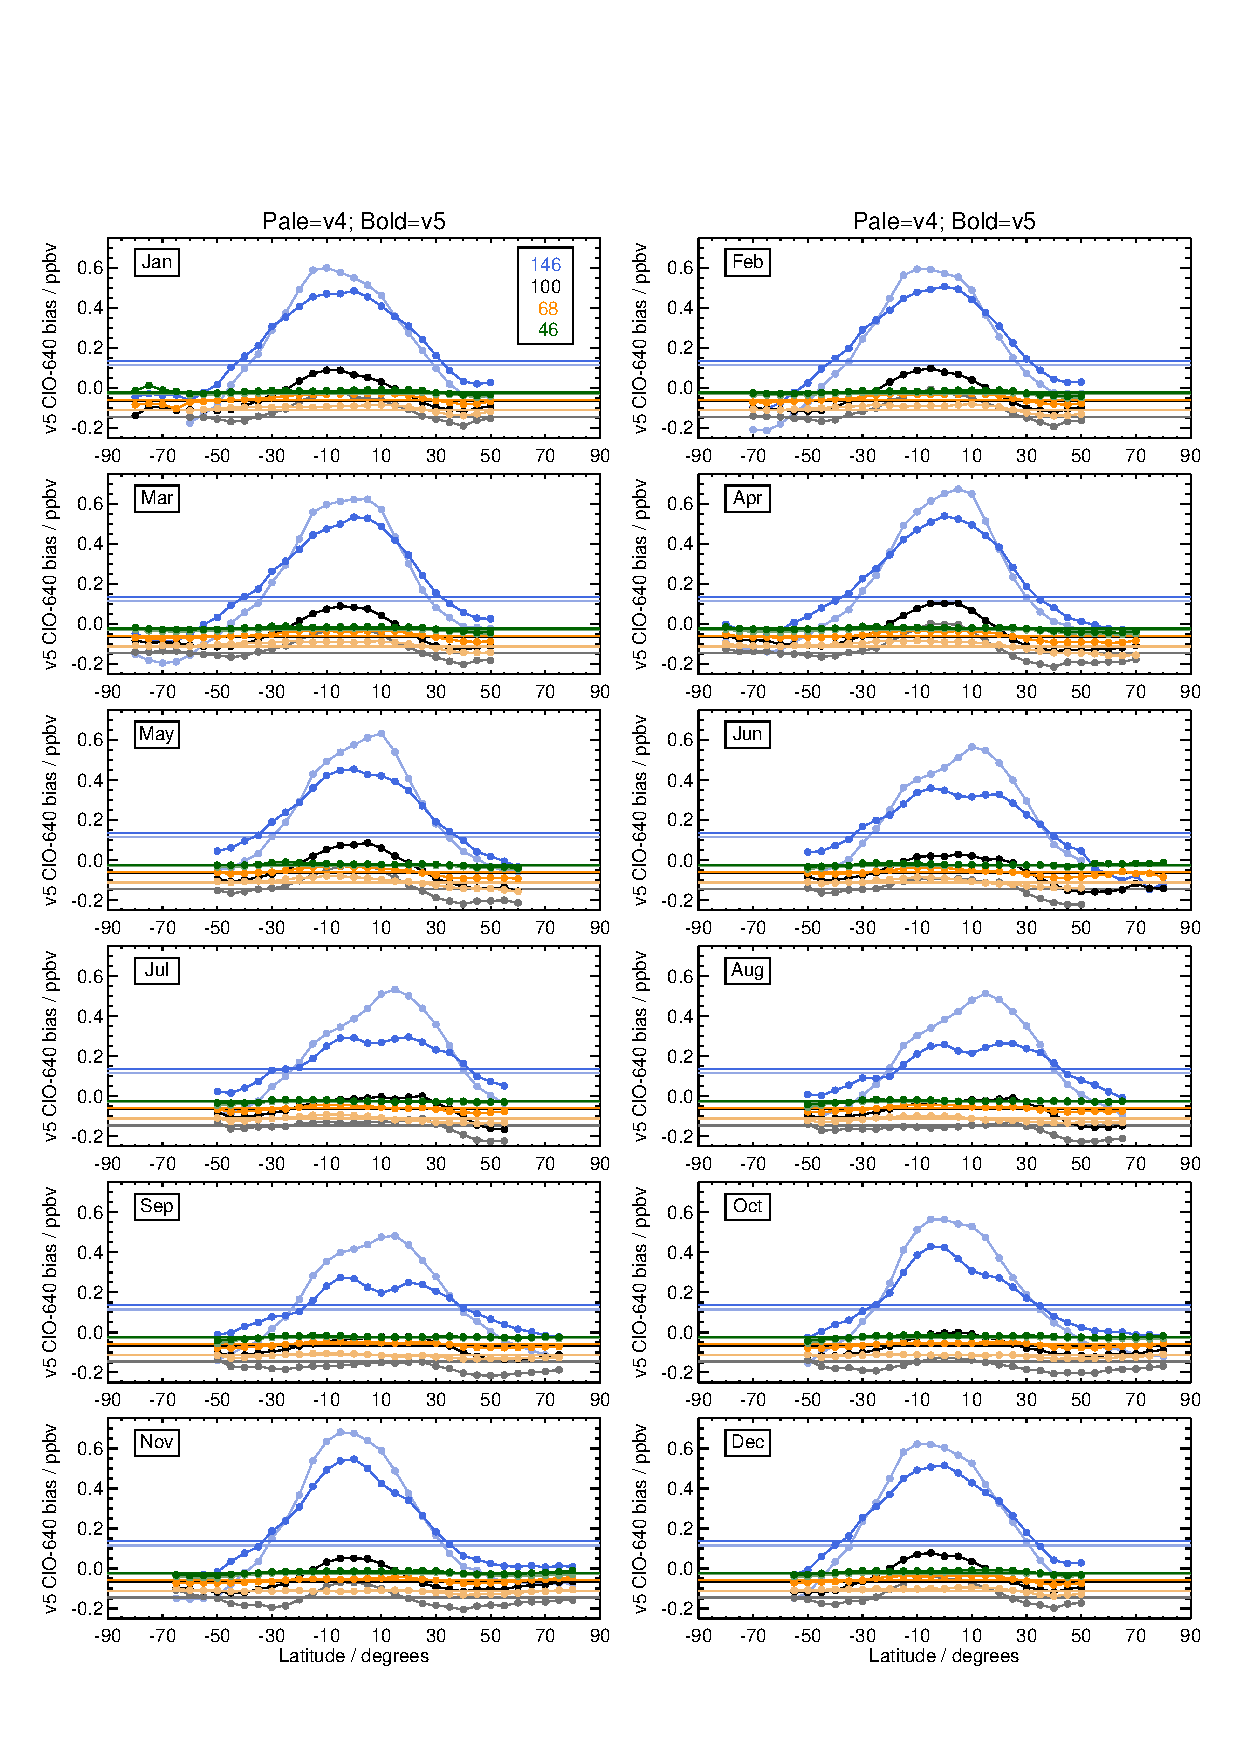
\includegraphics[width=\linewidth]{figures/plotBiasV5ByMonth-Clim_2020_ClO640}
\caption{Estimates of the bias in MLS \thisv ClO data in
  5{\degsym}-wide geographic latitude bands on the 147, 100, 68, and
  46\,hPa MLS retrieval pressure surfaces (see legend).  Each panel
  shows monthly zonal means of \thisv MLS nighttime (solar zenith
  angle $>$ 100{\degsym}) ClO measurements averaged over a
  \mbox{16-yr} period (2005--2020, filled circles). Results for \thisv
  are depicted in bold colors, those for \prevv in corresponding pale
  colors.  The horizontal lines denote the global-mean annual-mean
  bias estimates over the climatological period for both versions at
  each level.  To ensure that ClO was not enhanced, consideration was
  restricted to latitudes equatorward of 50{\degsym}S for the days
  between 1~May and 1~November and to latitudes equatorward of
  50{\degsym}N for the days between 1~December and 1~April.}
\label{fig:cloBiasByMonth}
\end{figure}

In many cases the ClO bias can be essentially eliminated by
subtracting daily gridded or zonal-mean nighttime values from daytime
measurements, and where feasible that is often the preferred
bias-correction approach.  However, it is not practical to do so under
conditions of continuous daylight in the summer or continuous darkness
in the winter at high latitudes.  Moreover, under certain
circumstances during the mid-winter period of peak ClO enhancement
inside the lower stratospheric polar vortices, non-negligible ClO
abundances can be present even in darkness, masking the negative bias.
In this case, computing day$-$night differences considerably reduces
the apparent degree of observed chlorine activation.  Consequently,
for studies of polar chemical processing and chlorine partitioning, it
is instead recommended that an estimate of the bias be subtracted from
the individual measurements at each affected retrieval level.
Attempts to estimate the bias through approaches other than
examination of nighttime ClO measurements (e.g., via correlations with
potentially interfering species, which themselves may vary strongly
with season) have so far met with limited success.  Thus the bias is
estimated from the analysis depicted in
Figure~\ref{fig:cloBiasByPress}.  Although monthly varying bias
estimates might be desirable, as noted above seasonal variations are
small, and it is not possible to directly quantify the bias in the
polar regions during much of the year.  Interannual variations and
longer-term trends (not shown) in the magnitude of the bias are also
small (especially in comparison to the uncertainty in the bias
estimates and the \thisv ClO data themselves; see
Section~\ref{sec:cloacc}).  For these reasons, and to simplify
application of the ClO bias correction for MLS data users, we report
\mbox{16-yr} climatological bias estimates that vary latitudinally and
altitudinally but not temporally; these bias corrections should be
adequate for most studies.  The bias values, reported on a 5{\degsym}
grid, must be interpolated to the MLS Level~2 measurement locations on
each day being considered and subtracted from the ClO mixing ratios
(daytime or nighttime) at those locations.  The bias correction must
be performed \emph{before} interpolation to a different vertical
coordinate (e.g., potential temperature). An ASCII file containing the
estimated ClO bias values has been embedded in the PDF version of this
document; instructions for extracting this file are given in
Appendix~\ref{appsec:ClO}.  The file is also available at
\url{https://mls.jpl.nasa.gov/data/MLS-Aura_ClO-BiasCorrection_v05.txt}.

\begin{figure}
\centering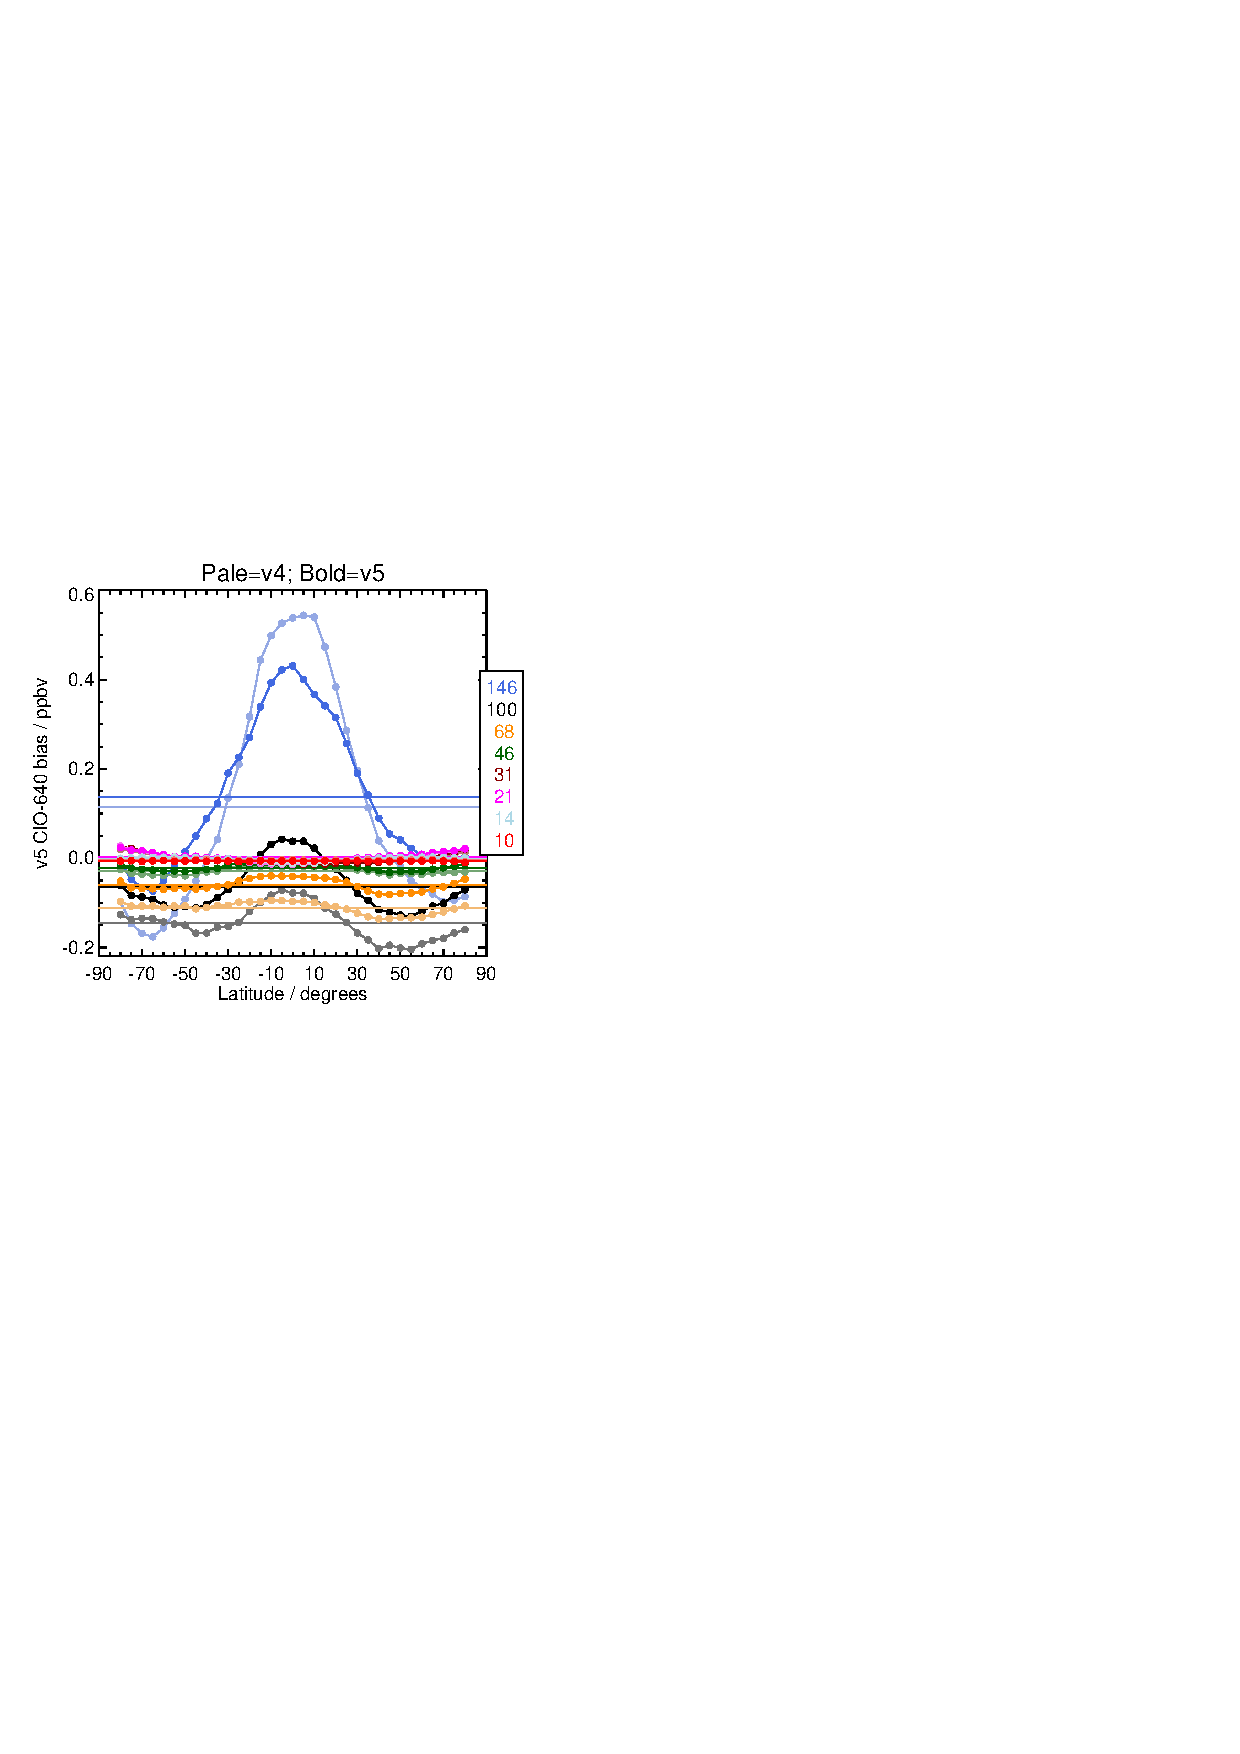
\includegraphics[width=0.6\linewidth,clip=true, trim=0cm 12.6cm 11.0cm 9.0cm]{figures/plotBiasV5-Clim_2020_ClO640}
%\centering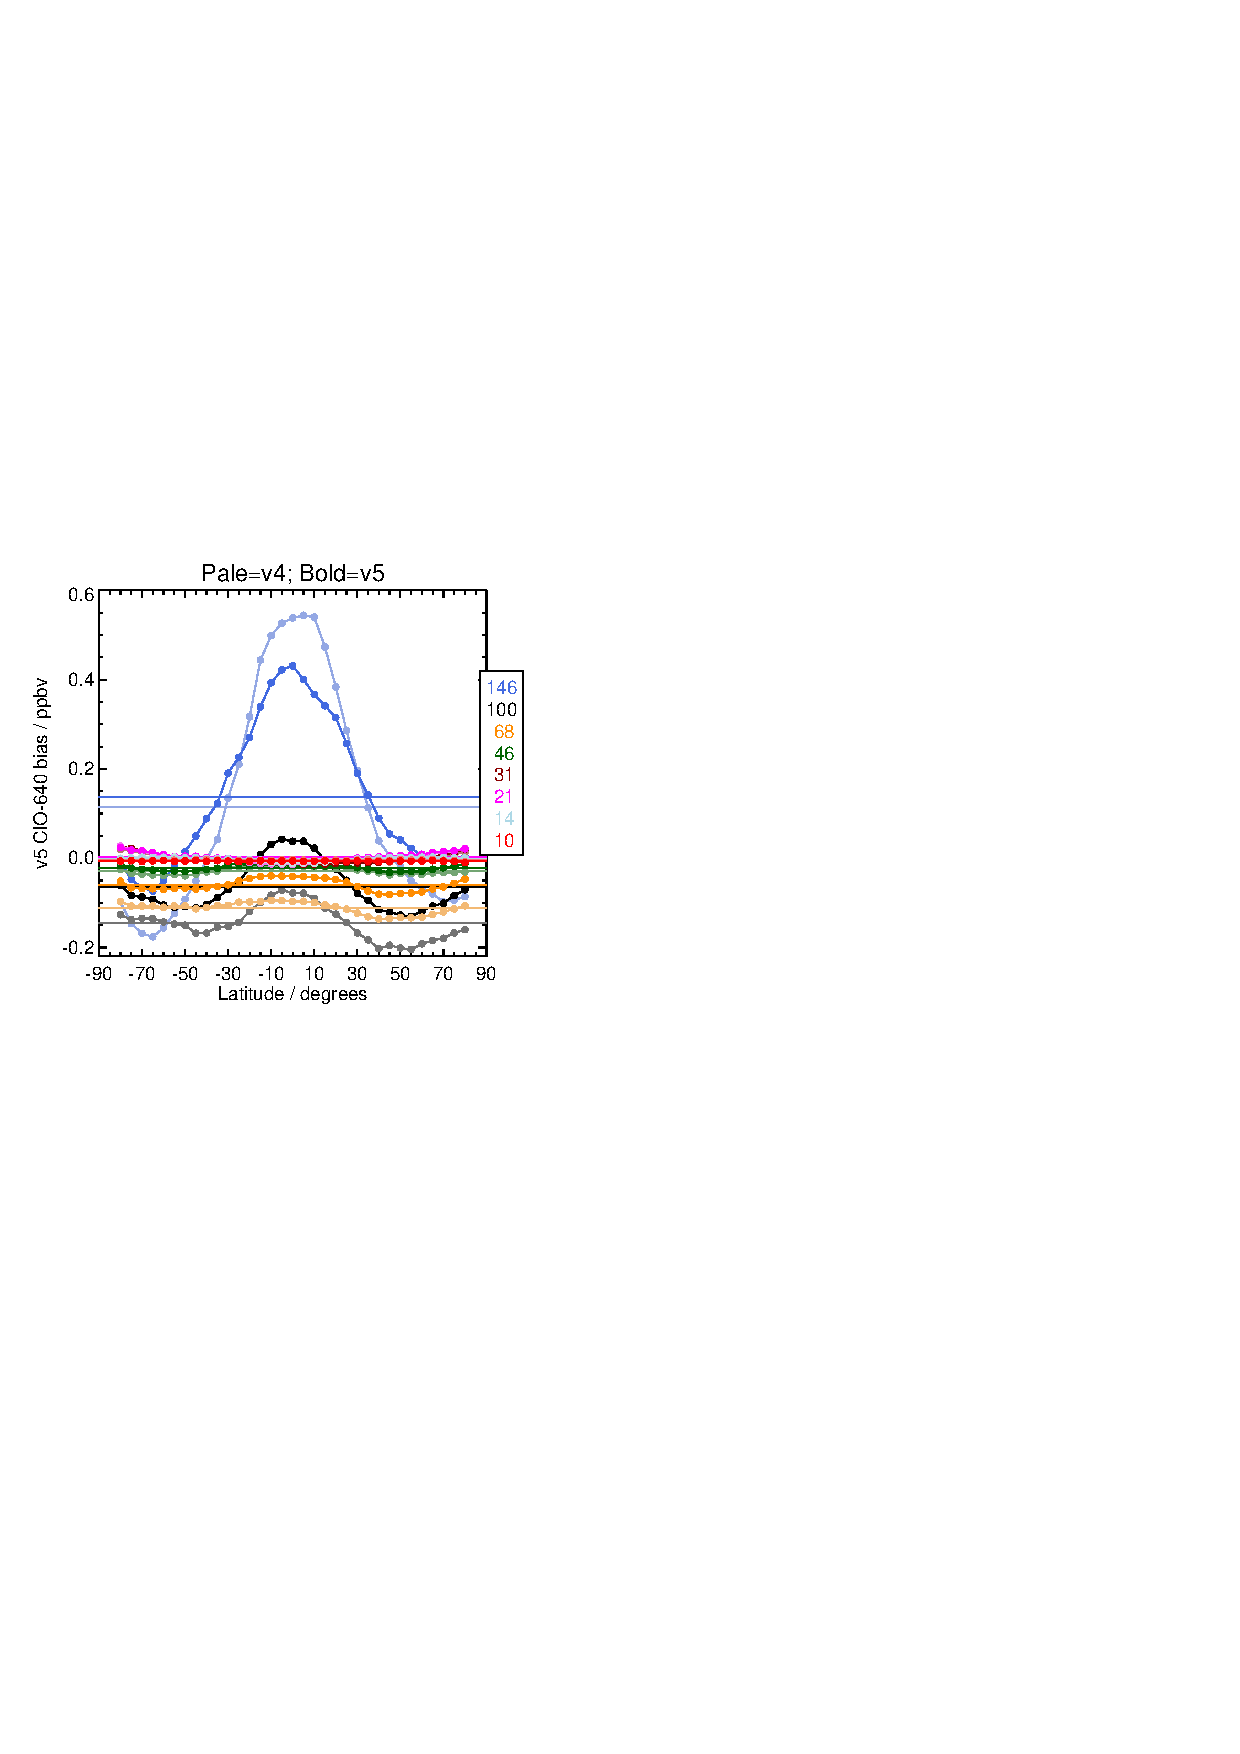
\includegraphics[width=\linewidth]{figures/plotBiasV5-Clim_2020_ClO640}
   \caption{Estimates of the bias in MLS \thisv nighttime (solar
     zenith angle $>$ 100{\degsym}) ClO data in 5{\degsym}-wide
     geographic latitude bands on MLS retrieval pressure surfaces from
     147 to 10\,hPa (see legend) calculated over a \mbox{16-yr} period
     (2005--2020).  Results for \thisv are depicted in bold colors,
     those for \prevv in corresponding pale colors.  The horizontal
     lines denote the global-mean annual-mean bias estimates over the
     climatological period for both versions at each level.  To ensure
     that ClO was not enhanced, consideration was restricted to
     latitudes equatorward of 50{\degsym}S for the days between 1~May
     and 1~November and to latitudes equatorward of 50{\degsym}N for
     the days between 1~December and 1~April.}
\label{fig:cloBiasByPress}
\end{figure}

\subsection{Review of comparisons with other  data sets}

Extensive comparisons of MLS v2.2 ClO data with measurements from a
variety of different platforms (ground-based, balloon-borne, aircraft,
and satellite) were presented by \citet{SanteeEtal:2008:ClO}.  A
subset of those comparisons with v3.3\emph{x}/v3.4\emph{x} ClO data
were reported by \citet{EOSMLSV33V34Quality}.  Comparisons of \thisv
ClO with correlative measurements have not been conducted but are
expected to yield results similar to those for previous versions.

\subsection{Data screening}
\label{sec:ClOScreening}
\begin{description}
\item[Pressure range:] \screeningrule{147--1.0\,hPa}
  \standardrangestatement

  \standardprecisionrule

\item[Status flag:] \screeningrule{Only use profiles for which the
  \texttt{Status} field is zero.}  

  We recommend that all profiles with nonzero values of
  \texttt{Status} be discarded, because of the potential impact of
  cloud artifacts at lower levels.  Note, however, that rejecting in
  their entirety all profiles with nonzero \texttt{Status} may be
  unnecessarily severe at and above (i.e., at pressures equal to or
  smaller than) 46\,hPa, where clouds have negligible impact; thus
  otherwise good-quality profiles with nonzero but even
  \texttt{Status} values may be used without restriction at those
  levels as long as they are removed at larger pressures.  See
  Section~\ref{sec:StatusQuality} for more information on the
  interpretation of the \texttt{Status} field.

\item[Quality:] \qualityrule{1.3} 

  This threshold for \texttt{Quality} (unchanged from \prevv)
  typically excludes less than 0.5\% of ClO profiles on a daily basis;
  note that it potentially discards some ``good'' data points while
  not necessarily identifying all ``bad'' ones.

\item[Convergence:] \convergencerule{1.05} 

  On a typical day this threshold for \texttt{Convergence} (unchanged
  from \prevv) discards very few (0.5\% or less) of the ClO profiles,
  many (but not all) of which are filtered out by the other quality
  control measures.
\end{description}

\subsection{Artifacts}
\begin{itemize}
\item Non-negligible biases are present in both daytime and nighttime
  \thisv ClO mixing ratios at and below (i.e., pressures larger than)
  68\,hPa.  The bias should be corrected by subtracting from the
  individual measurements at each affected retrieval level the
  altitude- and latitude-dependent bias estimates reported in an ASCII
  file that has been embedded in the PDF version of this document;
  instructions for extracting this file are given in
  Appendix~\ref{appsec:ClO}.  This file is also available at
  \url{https://mls.jpl.nasa.gov/data/MLS-Aura_ClO-BiasCorrection_v05.txt}.
\item Care must be taken in interpreting the ClO measurements
  immediately following severe pyrocumulonimbus (pyroCbs) events,
  which can rapidly loft polluted air from the surface and deposit it
  in the lower stratosphere.  Air masses characterized by enhanced
  abundances of biomass burning pollutants may appear to also contain
  elevated levels of ClO, but such apparent enhancements are artifacts
  induced by contamination of the ClO retrieval from methanol
  (CH\cs3OH), a product of wildfires that has a similar spectral
  signature in the MLS band used to measure ClO\@.
\end{itemize}

\subsection{Desired improvements for future data version(s)}
\begin{itemize}
\item Reduce the biases present at the lowest retrieval levels
  (147--68\,hPa).
\end{itemize}

\begin{DIFnomarkup}
\begin{table*}[bp]
\caption{Summary of Aura MLS \thisv ClO Characteristics}\vspace{0.5ex}
\label{tab:ClOSummary}
\begin{minipage}{\linewidth}\small
\renewcommand{\thefootnote}{\thempfootnote}
\centering\begin{tabular}{ccccl}
\toprule
\parbox[m]{18mm}{\bfseries\centering{Pressure\\ / hPa}} &
\parbox[m]{24mm}{\bfseries\centering{Resolution\\ V $\times$ H%
\footnote{Vertical and Horizontal resolution in along-track direction.} \\ / km}} &
\parbox[m]{17mm}{\bfseries\centering{Precision%
\footnote{Precision on individual profiles, determined from observed
 scatter in nighttime (descending) data in a region of minimal atmospheric
 variability.} \\/ ppbv}} &
\parbox[m]{20mm}{\bfseries\centering{Systematic\\ Uncertainty%
    \footnote{Values should be interpreted as \mbox{2-$\sigma$}
      estimates of the probable magnitude and, at the higher
      pressures, are the uncertainties after subtraction of the known
      bias.}\gdef\fnTwoSigma{\value{mpfootnote}}\\ / ppbv}} &
\parbox[m]{40mm}{\bfseries\centering{Known Artifacts\\ or Other Comments}} \\
%
\midrule
%
0.68--0.001 & ---   & ---  & ---  &  Unsuitable for scientific use\\
%
1.0         & 3        $\times$ 500      & $\pm$0.3 & $\pm$0.02 & \\
%
6.8--1.5    & 3.5--4   $\times$ 250--350 & $\pm$0.1 & $\pm$0.02 & \\
%
15--10     & 3.5   $\times$ 250 & $\pm$0.1 & $\pm$0.03 & \\
%
22          & 3        $\times$ 300      & $\pm$0.1 & $\pm$0.05  & \\
%
46--32      & 3        $\times$ 300--400 & $\pm$0.1 & $\pm$0.15  & \\
%
68 & 3 $\times$ 450 & $\pm$0.1 & $\pm$0.2 & Latitude-dependent
bias\footnote{Correct for the bias by subtracting from the individual
  measurements at this level the latitude-dependent bias estimates
  (see Section~\ref{sec:cloBias}).}\gdef\fnDirect{\value{mpfootnote}} \\
%
100         & 3        $\times$ 500      & $\pm$0.1 & $\pm$0.3  & 
Latitude-dependent bias\footnotemark[\fnDirect] \\
%
147         & 4.5      $\times$ 650      & $\pm$0.2 & $\pm$0.6  & 
Latitude-dependent bias\footnotemark[\fnDirect] \\
%
1000--215   & ---   & ---   & --- &  Not retrieved\\
%
\bottomrule
\end{tabular}
\end{minipage}
\end{table*}
\end{DIFnomarkup}

%%% Local Variables: 
%%% mode: latex
%%% TeX-master: "v5-x-report"
%%% End: 

